\chapter{Grafika (II qism): TikZ, PGFPlots va geometriya chizmalari}

\section{Lecture notes rejasi}
Bu bob “amaliy topshiriq” emas. Maqsad: \LaTeX{} ichida grafikani
tizimli o‘rganish va qayta ishlatish (reusable) shablonlar yaratish.
Har bir misolda \textbf{kod} va \textbf{natija} yonma-yon beriladi.

\section{TikZ operatorlari: minimal yadro}
\begin{enumerate}
\item Midpoint: \code{($(A)!0.5!(B)$)}
\item Ratio division: \code{($(A)!t!(B)$)}
\item Projection: \code{($(A)!(P)!(B)$)}
\item Intersection: \code{name path} + \code{name intersections}
\item Circle-through: \code{(O) circle through (A)}
\item Angle mark: \code{\textbackslash pic \{angle=...\}}
\end{enumerate}

\subsection{F1) Uchburchak + balandlik oyoği (projection)}
Projection: \code{($(A)!(C)!(B)$)} nuqta $C$ ning $AB$ ga proyeksiyasini beradi.

\begin{figure}[H]
\centering
\begin{minipage}{0.56\linewidth}
\begin{lstlisting}
\begin{tikzpicture}
\coordinate (A) at (0,0);
\coordinate (B) at (4,0);
\coordinate (C) at (1.2,2.6);
\draw[thick] (A)--(B)--(C)--cycle;
\coordinate (H) at ($(A)!(C)!(B)$);
\draw[dashed] (C)--(H);
\fill (A) circle(1.3pt) node[below left]{$A$};
\fill (B) circle(1.3pt) node[below right]{$B$};
\fill (C) circle(1.3pt) node[above]{$C$};
\fill (H) circle(1.3pt) node[below]{$H$};
\end{tikzpicture}
\end{lstlisting}
\end{minipage}\hfill
\begin{minipage}{0.40\linewidth}
\centering
\begin{tikzpicture}
\coordinate (A) at (0,0);
\coordinate (B) at (4,0);
\coordinate (C) at (1.2,2.6);
\draw[thick] (A)--(B)--(C)--cycle;
\coordinate (H) at ($(A)!(C)!(B)$);
\draw[dashed] (C)--(H);
\fill (A) circle(1.3pt) node[below left]{$A$};
\fill (B) circle(1.3pt) node[below right]{$B$};
\fill (C) circle(1.3pt) node[above]{$C$};
\fill (H) circle(1.3pt) node[below]{$H$};
\end{tikzpicture}
\end{minipage}
\caption{Projection operator bilan $H$ proyeksiya oyoği.}\label{fig:F1}
\end{figure}
\FloatBarrier
\clearpage

\section{Uchburchak markazlari: $G,H,I,O$}\n
\subsection{C1) Centroid $G$ (medianlar kesishmasi)}
\begin{figure}[H]
\centering
\begin{minipage}{0.56\linewidth}
\begin{lstlisting}
\begin{tikzpicture}
\coordinate (A) at (0,0);
\coordinate (B) at (5,0);
\coordinate (C) at (1.6,3.1);
\draw[thick] (A)--(B)--(C)--cycle;
\coordinate (Mbc) at ($(B)!0.5!(C)$);
\coordinate (Mca) at ($(C)!0.5!(A)$);
\path[name path=medA] (A)--(Mbc);
\path[name path=medB] (B)--(Mca);
\draw[dashed] (A)--(Mbc);
\draw[dashed] (B)--(Mca);
\path[name intersections={of=medA and medB, by=G}];
\fill (G) circle(1.6pt) node[above right]{$G$};
\end{tikzpicture}
\end{lstlisting}
\end{minipage}\hfill
\begin{minipage}{0.40\linewidth}
\centering
\begin{tikzpicture}
\coordinate (A) at (0,0);
\coordinate (B) at (5,0);
\coordinate (C) at (1.6,3.1);
\draw[thick] (A)--(B)--(C)--cycle;
\coordinate (Mbc) at ($(B)!0.5!(C)$);
\coordinate (Mca) at ($(C)!0.5!(A)$);
\path[name path=medA] (A)--(Mbc);
\path[name path=medB] (B)--(Mca);
\draw[dashed] (A)--(Mbc);
\draw[dashed] (B)--(Mca);
\path[name intersections={of=medA and medB, by=G}];
\fill (G) circle(1.6pt) node[above right]{$G$};
\end{tikzpicture}
\end{minipage}
\caption{Ikki median kesishmasidan $G$ olinadi.}\label{fig:C1}
\end{figure}
\FloatBarrier
\clearpage

\subsection{C2) Orthocenter $H$ (balandliklar kesishmasi)}
\begin{figure}[H]
\centering
\begin{minipage}{0.56\linewidth}
\begin{lstlisting}
\begin{tikzpicture}
\coordinate (A) at (0,0);
\coordinate (B) at (5,0);
\coordinate (C) at (1.5,3.2);
\draw[thick] (A)--(B)--(C)--cycle;
\coordinate (Ha) at ($(B)!(A)!(C)$);
\coordinate (Hb) at ($(C)!(B)!(A)$);
\path[name path=hA] (A)--(Ha);
\path[name path=hB] (B)--(Hb);
\draw[dashed] (A)--(Ha);
\draw[dashed] (B)--(Hb);
\path[name intersections={of=hA and hB, by=H}];
\fill (H) circle(1.6pt) node[above right]{$H$};
\end{tikzpicture}
\end{lstlisting}
\end{minipage}\hfill
\begin{minipage}{0.40\linewidth}
\centering
\begin{tikzpicture}
\coordinate (A) at (0,0);
\coordinate (B) at (5,0);
\coordinate (C) at (1.5,3.2);
\draw[thick] (A)--(B)--(C)--cycle;
\coordinate (Ha) at ($(B)!(A)!(C)$);
\coordinate (Hb) at ($(C)!(B)!(A)$);
\path[name path=hA] (A)--(Ha);
\path[name path=hB] (B)--(Hb);
\draw[dashed] (A)--(Ha);
\draw[dashed] (B)--(Hb);
\path[name intersections={of=hA and hB, by=H}];
\fill (H) circle(1.6pt) node[above right]{$H$};
\end{tikzpicture}
\end{minipage}
\caption{Ikki balandlik kesishmasidan $H$ olinadi.}\label{fig:C2}
\end{figure}
\FloatBarrier
\clearpage

\subsection{C3) Incenter $I$ va incircle}
\begin{figure}[H]
\centering
\begin{minipage}{0.56\linewidth}
\begin{lstlisting}
\begin{tikzpicture}
\coordinate (A) at (0,0);
\coordinate (B) at (5,0);
\coordinate (C) at (1.4,3.0);
\draw[thick] (A)--(B)--(C)--cycle;
\path let \p1=(B), \p2=(C), \p3=(C), \p4=(A), \p5=(A), \p6=(B) in
  \pgfextra{
    \pgfmathsetmacro{\a}{veclen(\x1-\x2,\y1-\y2)}
    \pgfmathsetmacro{\b}{veclen(\x3-\x4,\y3-\y4)}
    \pgfmathsetmacro{\c}{veclen(\x5-\x6,\y5-\y6)}
  };
\coordinate (I) at (barycentric cs:A=\a,B=\b,C=\c);
\coordinate (T) at ($(A)!(I)!(B)$);
\draw[dashed] (I)--(T);
\draw[thick] (I) circle through (T);
\fill (I) circle(1.6pt) node[above right]{$I$};
\end{tikzpicture}
\end{lstlisting}
\end{minipage}\hfill
\begin{minipage}{0.40\linewidth}
\centering
\begin{tikzpicture}
\coordinate (A) at (0,0);
\coordinate (B) at (5,0);
\coordinate (C) at (1.4,3.0);
\draw[thick] (A)--(B)--(C)--cycle;
\path let \p1=(B), \p2=(C), \p3=(C), \p4=(A), \p5=(A), \p6=(B) in
  \pgfextra{
    \pgfmathsetmacro{\a}{veclen(\x1-\x2,\y1-\y2)}
    \pgfmathsetmacro{\b}{veclen(\x3-\x4,\y3-\y4)}
    \pgfmathsetmacro{\c}{veclen(\x5-\x6,\y5-\y6)}
  };
\coordinate (I) at (barycentric cs:A=\a,B=\b,C=\c);
\coordinate (T) at ($(A)!(I)!(B)$);
\draw[dashed] (I)--(T);
\draw[thick] (I) circle through (T);
\fill (I) circle(1.6pt) node[above right]{$I$};
\end{tikzpicture}
\end{minipage}
\caption{Barycentric cs (tomon uzunliklari) + circle through.}\label{fig:C3}
\end{figure}
\FloatBarrier
\clearpage

\subsection{C4) Circumcenter $O$ va circumcircle}
\begin{figure}[H]
\centering
\begin{minipage}{0.56\linewidth}
\begin{lstlisting}
\begin{tikzpicture}
\coordinate (A) at (0,0);
\coordinate (B) at (5,0);
\coordinate (C) at (1.6,3.2);
\draw[thick] (A)--(B)--(C)--cycle;
\coordinate (Mab) at ($(A)!0.5!(B)$);
\coordinate (Mbc) at ($(B)!0.5!(C)$);
\coordinate (Pab) at ($(Mab)!1!90:(B)$);
\coordinate (Pbc) at ($(Mbc)!1!90:(C)$);
\path[name path=pb1] (Mab)--(Pab);
\path[name path=pb2] (Mbc)--(Pbc);
\draw[dashed] (Mab)--(Pab);
\draw[dashed] (Mbc)--(Pbc);
\path[name intersections={of=pb1 and pb2, by=O}];
\draw[thick] (O) circle through (A);
\fill (O) circle(1.6pt) node[above right]{$O$};
\end{tikzpicture}
\end{lstlisting}
\end{minipage}\hfill
\begin{minipage}{0.40\linewidth}
\centering
\begin{tikzpicture}
\coordinate (A) at (0,0);
\coordinate (B) at (5,0);
\coordinate (C) at (1.6,3.2);
\draw[thick] (A)--(B)--(C)--cycle;
\coordinate (Mab) at ($(A)!0.5!(B)$);
\coordinate (Mbc) at ($(B)!0.5!(C)$);
\coordinate (Pab) at ($(Mab)!1!90:(B)$);
\coordinate (Pbc) at ($(Mbc)!1!90:(C)$);
\path[name path=pb1] (Mab)--(Pab);
\path[name path=pb2] (Mbc)--(Pbc);
\draw[dashed] (Mab)--(Pab);
\draw[dashed] (Mbc)--(Pbc);
\path[name intersections={of=pb1 and pb2, by=O}];
\draw[thick] (O) circle through (A);
\fill (O) circle(1.6pt) node[above right]{$O$};
\end{tikzpicture}
\end{minipage}
\caption{Perpendikulyar o‘rtachilar kesishmasi + circle through (A).}\label{fig:C4}
\end{figure}
\FloatBarrier
\clearpage

\section{Katta katalog: 70 ta chizma (har biri alohida sahifada)}

\subsection{G1) Geometriya chizmasi 1}
Chapda kod, o‘ngda natija. TikZ’ni odat bo‘yicha: koordinata → asosiy chiziqlar → yordamchi chiziqlar → belgilash.

\begin{figure}[H]
\centering
\begin{minipage}{0.56\linewidth}
\begin{lstlisting}
\begin{tikzpicture}
\coordinate (A) at (0,0);\coordinate (B) at (5,0);
\coordinate (P) at ($(A)!0.3!(B)$);
\draw[thick] (A)--(B);
\fill (A) circle(1.2pt) node[below]{$A$};
\fill (B) circle(1.2pt) node[below]{$B$};
\fill (P) circle(1.5pt) node[below]{$P$};
\end{tikzpicture}
\end{lstlisting}
\end{minipage}\hfill
\begin{minipage}{0.40\linewidth}
\centering
\begin{tikzpicture}
\coordinate (A) at (0,0);\coordinate (B) at (5,0);
\coordinate (P) at ($(A)!0.3!(B)$);
\draw[thick] (A)--(B);
\fill (A) circle(1.2pt) node[below]{$A$};
\fill (B) circle(1.2pt) node[below]{$B$};
\fill (P) circle(1.5pt) node[below]{$P$};
\end{tikzpicture}
\end{minipage}
\caption{Kesmani ratio orqali bo‘lish: $P=(A)!0.3!(B)$. }\label{fig:G1}
\end{figure}
\FloatBarrier
\clearpage

\subsection{G2) Geometriya chizmasi 2}
Chapda kod, o‘ngda natija. TikZ’ni odat bo‘yicha: koordinata → asosiy chiziqlar → yordamchi chiziqlar → belgilash.

\begin{figure}[H]
\centering
\begin{minipage}{0.56\linewidth}
\begin{lstlisting}
\begin{tikzpicture}
\coordinate (A) at (0,0);\coordinate (B) at (4,1);
\coordinate (P) at (0.6,2.2);
\coordinate (Q) at ($(P)+(B)-(A)$);
\draw[thick] (A)--(B);
\draw[dashed, thick] (P)--(Q);
\fill (P) circle(1.2pt) node[left]{$P$};
\end{tikzpicture}
\end{lstlisting}
\end{minipage}\hfill
\begin{minipage}{0.40\linewidth}
\centering
\begin{tikzpicture}
\coordinate (A) at (0,0);\coordinate (B) at (4,1);
\coordinate (P) at (0.6,2.2);
\coordinate (Q) at ($(P)+(B)-(A)$);
\draw[thick] (A)--(B);
\draw[dashed, thick] (P)--(Q);
\fill (P) circle(1.2pt) node[left]{$P$};
\end{tikzpicture}
\end{minipage}
\caption{Parallel ko‘chirish: $Q=P+(B-A)$. }\label{fig:G2}
\end{figure}
\FloatBarrier
\clearpage

\subsection{G3) Geometriya chizmasi 3}
Chapda kod, o‘ngda natija. TikZ’ni odat bo‘yicha: koordinata → asosiy chiziqlar → yordamchi chiziqlar → belgilash.

\begin{figure}[H]
\centering
\begin{minipage}{0.56\linewidth}
\begin{lstlisting}
\begin{tikzpicture}
\coordinate (A) at (0,0);\coordinate (B) at (4,0.8);
\draw[thick] (A)--(B);
\coordinate (M) at ($(A)!0.5!(B)$);
\coordinate (R) at ($(M)!2!90:(B)$);
\draw[dashed, thick] (M)--(R);
\fill (M) circle(1.2pt) node[below]{$M$};
\end{tikzpicture}
\end{lstlisting}
\end{minipage}\hfill
\begin{minipage}{0.40\linewidth}
\centering
\begin{tikzpicture}
\coordinate (A) at (0,0);\coordinate (B) at (4,0.8);
\draw[thick] (A)--(B);
\coordinate (M) at ($(A)!0.5!(B)$);
\coordinate (R) at ($(M)!2!90:(B)$);
\draw[dashed, thick] (M)--(R);
\fill (M) circle(1.2pt) node[below]{$M$};
\end{tikzpicture}
\end{minipage}
\caption{Perpendikulyar o‘rtachi skeleti. }\label{fig:G3}
\end{figure}
\FloatBarrier
\clearpage

\subsection{G4) Geometriya chizmasi 4}
Chapda kod, o‘ngda natija. TikZ’ni odat bo‘yicha: koordinata → asosiy chiziqlar → yordamchi chiziqlar → belgilash.

\begin{figure}[H]
\centering
\begin{minipage}{0.56\linewidth}
\begin{lstlisting}
\begin{tikzpicture}
\coordinate (A) at (0,0);\coordinate (B) at (4,2);
\coordinate (C) at (0,2);\coordinate (D) at (4,0);
\path[name path=l1] (A)--(B);
\path[name path=l2] (C)--(D);
\draw[thick] (A)--(B);
\draw[thick] (C)--(D);
\path[name intersections={of=l1 and l2, by=X}];
\fill (X) circle(1.5pt) node[above right]{$X$};
\end{tikzpicture}
\end{lstlisting}
\end{minipage}\hfill
\begin{minipage}{0.40\linewidth}
\centering
\begin{tikzpicture}
\coordinate (A) at (0,0);\coordinate (B) at (4,2);
\coordinate (C) at (0,2);\coordinate (D) at (4,0);
\path[name path=l1] (A)--(B);
\path[name path=l2] (C)--(D);
\draw[thick] (A)--(B);
\draw[thick] (C)--(D);
\path[name intersections={of=l1 and l2, by=X}];
\fill (X) circle(1.5pt) node[above right]{$X$};
\end{tikzpicture}
\end{minipage}
\caption{name path + intersections. }\label{fig:G4}
\end{figure}
\FloatBarrier
\clearpage

\subsection{G5) Geometriya chizmasi 5}
Chapda kod, o‘ngda natija. TikZ’ni odat bo‘yicha: koordinata → asosiy chiziqlar → yordamchi chiziqlar → belgilash.

\begin{figure}[H]
\centering
\begin{minipage}{0.56\linewidth}
\begin{lstlisting}
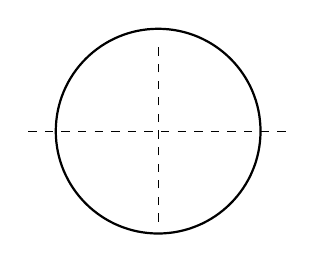
\begin{tikzpicture}
\draw[thick] (0,0) circle (1.30);
\draw[dashed] (-1.65,0)--(1.65,0);
\draw[dashed] (0,-1.15)--(0,1.15);
\end{tikzpicture}
\end{lstlisting}
\end{minipage}\hfill
\begin{minipage}{0.40\linewidth}
\centering
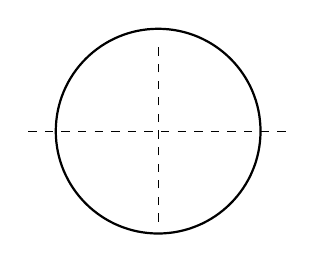
\begin{tikzpicture}
\draw[thick] (0,0) circle (1.30);
\draw[dashed] (-1.65,0)--(1.65,0);
\draw[dashed] (0,-1.15)--(0,1.15);
\end{tikzpicture}
\end{minipage}
\caption{Aylana + diametrlar (variant 5).}\label{fig:G5}
\end{figure}
\FloatBarrier
\clearpage

\subsection{G6) Geometriya chizmasi 6}
Chapda kod, o‘ngda natija. TikZ’ni odat bo‘yicha: koordinata → asosiy chiziqlar → yordamchi chiziqlar → belgilash.

\begin{figure}[H]
\centering
\begin{minipage}{0.56\linewidth}
\begin{lstlisting}
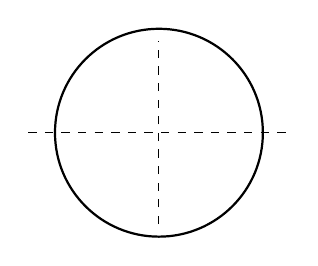
\begin{tikzpicture}
\draw[thick] (0,0) circle (1.32);
\draw[dashed] (-1.66,0)--(1.66,0);
\draw[dashed] (0,-1.16)--(0,1.16);
\end{tikzpicture}
\end{lstlisting}
\end{minipage}\hfill
\begin{minipage}{0.40\linewidth}
\centering
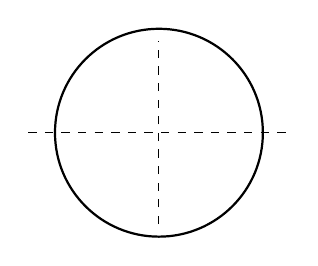
\begin{tikzpicture}
\draw[thick] (0,0) circle (1.32);
\draw[dashed] (-1.66,0)--(1.66,0);
\draw[dashed] (0,-1.16)--(0,1.16);
\end{tikzpicture}
\end{minipage}
\caption{Aylana + diametrlar (variant 6).}\label{fig:G6}
\end{figure}
\FloatBarrier
\clearpage

\subsection{G7) Geometriya chizmasi 7}
Chapda kod, o‘ngda natija. TikZ’ni odat bo‘yicha: koordinata → asosiy chiziqlar → yordamchi chiziqlar → belgilash.

\begin{figure}[H]
\centering
\begin{minipage}{0.56\linewidth}
\begin{lstlisting}
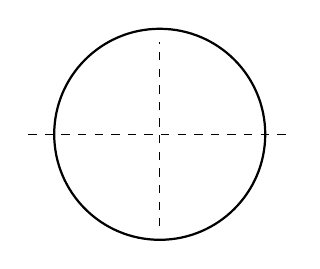
\begin{tikzpicture}
\draw[thick] (0,0) circle (1.34);
\draw[dashed] (-1.67,0)--(1.67,0);
\draw[dashed] (0,-1.17)--(0,1.17);
\end{tikzpicture}
\end{lstlisting}
\end{minipage}\hfill
\begin{minipage}{0.40\linewidth}
\centering
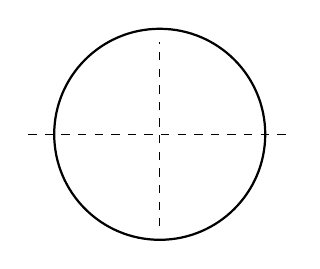
\begin{tikzpicture}
\draw[thick] (0,0) circle (1.34);
\draw[dashed] (-1.67,0)--(1.67,0);
\draw[dashed] (0,-1.17)--(0,1.17);
\end{tikzpicture}
\end{minipage}
\caption{Aylana + diametrlar (variant 7).}\label{fig:G7}
\end{figure}
\FloatBarrier
\clearpage

\subsection{G8) Geometriya chizmasi 8}
Chapda kod, o‘ngda natija. TikZ’ni odat bo‘yicha: koordinata → asosiy chiziqlar → yordamchi chiziqlar → belgilash.

\begin{figure}[H]
\centering
\begin{minipage}{0.56\linewidth}
\begin{lstlisting}
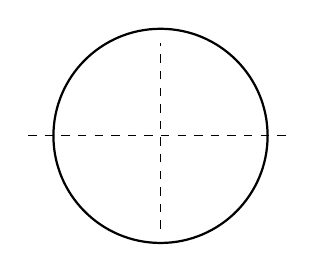
\begin{tikzpicture}
\draw[thick] (0,0) circle (1.36);
\draw[dashed] (-1.68,0)--(1.68,0);
\draw[dashed] (0,-1.18)--(0,1.18);
\end{tikzpicture}
\end{lstlisting}
\end{minipage}\hfill
\begin{minipage}{0.40\linewidth}
\centering
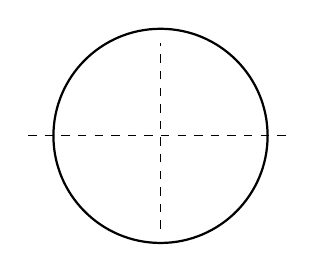
\begin{tikzpicture}
\draw[thick] (0,0) circle (1.36);
\draw[dashed] (-1.68,0)--(1.68,0);
\draw[dashed] (0,-1.18)--(0,1.18);
\end{tikzpicture}
\end{minipage}
\caption{Aylana + diametrlar (variant 8).}\label{fig:G8}
\end{figure}
\FloatBarrier
\clearpage

\subsection{G9) Geometriya chizmasi 9}
Chapda kod, o‘ngda natija. TikZ’ni odat bo‘yicha: koordinata → asosiy chiziqlar → yordamchi chiziqlar → belgilash.

\begin{figure}[H]
\centering
\begin{minipage}{0.56\linewidth}
\begin{lstlisting}
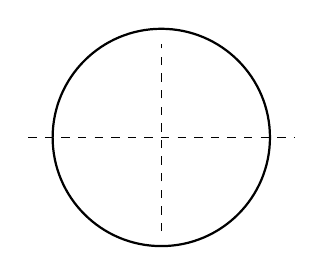
\begin{tikzpicture}
\draw[thick] (0,0) circle (1.38);
\draw[dashed] (-1.69,0)--(1.69,0);
\draw[dashed] (0,-1.19)--(0,1.19);
\end{tikzpicture}
\end{lstlisting}
\end{minipage}\hfill
\begin{minipage}{0.40\linewidth}
\centering
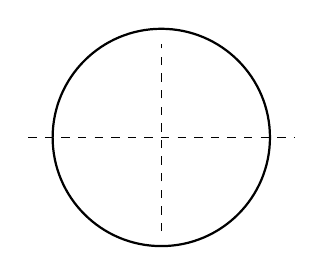
\begin{tikzpicture}
\draw[thick] (0,0) circle (1.38);
\draw[dashed] (-1.69,0)--(1.69,0);
\draw[dashed] (0,-1.19)--(0,1.19);
\end{tikzpicture}
\end{minipage}
\caption{Aylana + diametrlar (variant 9).}\label{fig:G9}
\end{figure}
\FloatBarrier
\clearpage

\subsection{G10) Geometriya chizmasi 10}
Chapda kod, o‘ngda natija. TikZ’ni odat bo‘yicha: koordinata → asosiy chiziqlar → yordamchi chiziqlar → belgilash.

\begin{figure}[H]
\centering
\begin{minipage}{0.56\linewidth}
\begin{lstlisting}
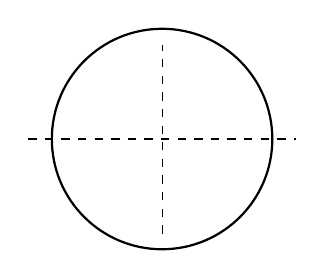
\begin{tikzpicture}
\draw[thick] (0,0) circle (1.40);
\draw[dashed] (-1.70,0)--(1.70,0);
\draw[dashed] (0,-1.20)--(0,1.20);
\end{tikzpicture}
\end{lstlisting}
\end{minipage}\hfill
\begin{minipage}{0.40\linewidth}
\centering
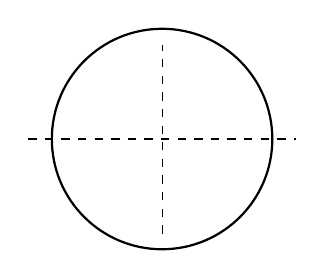
\begin{tikzpicture}
\draw[thick] (0,0) circle (1.40);
\draw[dashed] (-1.70,0)--(1.70,0);
\draw[dashed] (0,-1.20)--(0,1.20);
\end{tikzpicture}
\end{minipage}
\caption{Aylana + diametrlar (variant 10).}\label{fig:G10}
\end{figure}
\FloatBarrier
\clearpage

\subsection{G11) Geometriya chizmasi 11}
Chapda kod, o‘ngda natija. TikZ’ni odat bo‘yicha: koordinata → asosiy chiziqlar → yordamchi chiziqlar → belgilash.

\begin{figure}[H]
\centering
\begin{minipage}{0.56\linewidth}
\begin{lstlisting}
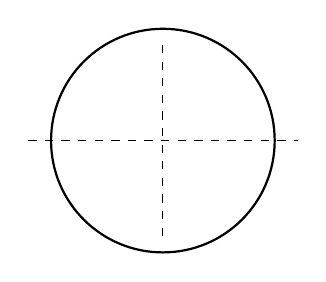
\begin{tikzpicture}
\draw[thick] (0,0) circle (1.42);
\draw[dashed] (-1.71,0)--(1.71,0);
\draw[dashed] (0,-1.21)--(0,1.21);
\end{tikzpicture}
\end{lstlisting}
\end{minipage}\hfill
\begin{minipage}{0.40\linewidth}
\centering
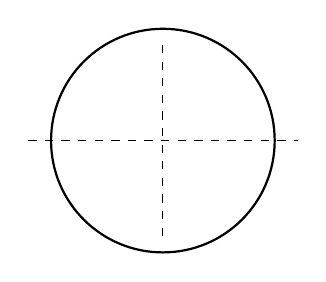
\begin{tikzpicture}
\draw[thick] (0,0) circle (1.42);
\draw[dashed] (-1.71,0)--(1.71,0);
\draw[dashed] (0,-1.21)--(0,1.21);
\end{tikzpicture}
\end{minipage}
\caption{Aylana + diametrlar (variant 11).}\label{fig:G11}
\end{figure}
\FloatBarrier
\clearpage

\subsection{G12) Geometriya chizmasi 12}
Chapda kod, o‘ngda natija. TikZ’ni odat bo‘yicha: koordinata → asosiy chiziqlar → yordamchi chiziqlar → belgilash.

\begin{figure}[H]
\centering
\begin{minipage}{0.56\linewidth}
\begin{lstlisting}
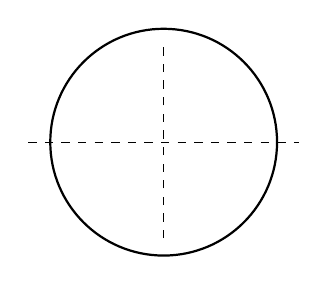
\begin{tikzpicture}
\draw[thick] (0,0) circle (1.44);
\draw[dashed] (-1.72,0)--(1.72,0);
\draw[dashed] (0,-1.22)--(0,1.22);
\end{tikzpicture}
\end{lstlisting}
\end{minipage}\hfill
\begin{minipage}{0.40\linewidth}
\centering
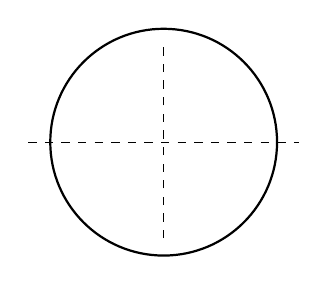
\begin{tikzpicture}
\draw[thick] (0,0) circle (1.44);
\draw[dashed] (-1.72,0)--(1.72,0);
\draw[dashed] (0,-1.22)--(0,1.22);
\end{tikzpicture}
\end{minipage}
\caption{Aylana + diametrlar (variant 12).}\label{fig:G12}
\end{figure}
\FloatBarrier
\clearpage

\subsection{G13) Geometriya chizmasi 13}
Chapda kod, o‘ngda natija. TikZ’ni odat bo‘yicha: koordinata → asosiy chiziqlar → yordamchi chiziqlar → belgilash.

\begin{figure}[H]
\centering
\begin{minipage}{0.56\linewidth}
\begin{lstlisting}
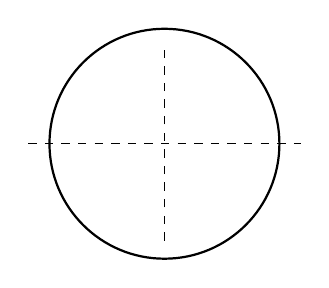
\begin{tikzpicture}
\draw[thick] (0,0) circle (1.46);
\draw[dashed] (-1.73,0)--(1.73,0);
\draw[dashed] (0,-1.23)--(0,1.23);
\end{tikzpicture}
\end{lstlisting}
\end{minipage}\hfill
\begin{minipage}{0.40\linewidth}
\centering
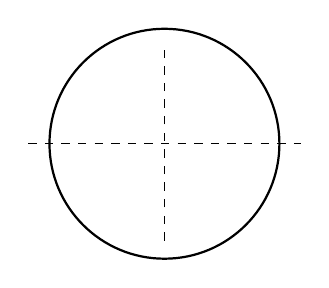
\begin{tikzpicture}
\draw[thick] (0,0) circle (1.46);
\draw[dashed] (-1.73,0)--(1.73,0);
\draw[dashed] (0,-1.23)--(0,1.23);
\end{tikzpicture}
\end{minipage}
\caption{Aylana + diametrlar (variant 13).}\label{fig:G13}
\end{figure}
\FloatBarrier
\clearpage

\subsection{G14) Geometriya chizmasi 14}
Chapda kod, o‘ngda natija. TikZ’ni odat bo‘yicha: koordinata → asosiy chiziqlar → yordamchi chiziqlar → belgilash.

\begin{figure}[H]
\centering
\begin{minipage}{0.56\linewidth}
\begin{lstlisting}
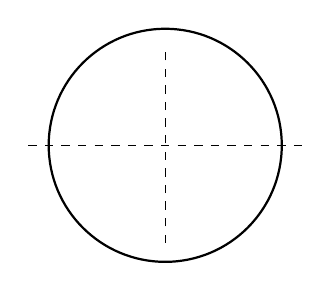
\begin{tikzpicture}
\draw[thick] (0,0) circle (1.48);
\draw[dashed] (-1.74,0)--(1.74,0);
\draw[dashed] (0,-1.24)--(0,1.24);
\end{tikzpicture}
\end{lstlisting}
\end{minipage}\hfill
\begin{minipage}{0.40\linewidth}
\centering
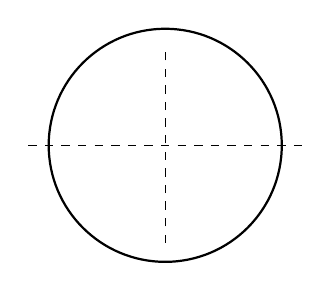
\begin{tikzpicture}
\draw[thick] (0,0) circle (1.48);
\draw[dashed] (-1.74,0)--(1.74,0);
\draw[dashed] (0,-1.24)--(0,1.24);
\end{tikzpicture}
\end{minipage}
\caption{Aylana + diametrlar (variant 14).}\label{fig:G14}
\end{figure}
\FloatBarrier
\clearpage

\subsection{G15) Geometriya chizmasi 15}
Chapda kod, o‘ngda natija. TikZ’ni odat bo‘yicha: koordinata → asosiy chiziqlar → yordamchi chiziqlar → belgilash.

\begin{figure}[H]
\centering
\begin{minipage}{0.56\linewidth}
\begin{lstlisting}
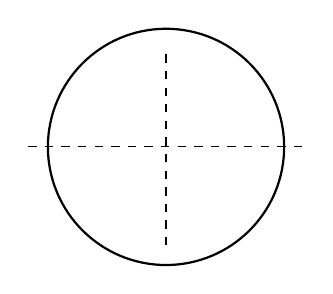
\begin{tikzpicture}
\draw[thick] (0,0) circle (1.50);
\draw[dashed] (-1.75,0)--(1.75,0);
\draw[dashed] (0,-1.25)--(0,1.25);
\end{tikzpicture}
\end{lstlisting}
\end{minipage}\hfill
\begin{minipage}{0.40\linewidth}
\centering
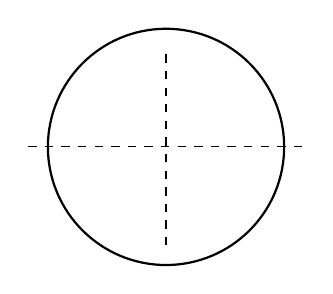
\begin{tikzpicture}
\draw[thick] (0,0) circle (1.50);
\draw[dashed] (-1.75,0)--(1.75,0);
\draw[dashed] (0,-1.25)--(0,1.25);
\end{tikzpicture}
\end{minipage}
\caption{Aylana + diametrlar (variant 15).}\label{fig:G15}
\end{figure}
\FloatBarrier
\clearpage

\subsection{G16) Geometriya chizmasi 16}
Chapda kod, o‘ngda natija. TikZ’ni odat bo‘yicha: koordinata → asosiy chiziqlar → yordamchi chiziqlar → belgilash.

\begin{figure}[H]
\centering
\begin{minipage}{0.56\linewidth}
\begin{lstlisting}
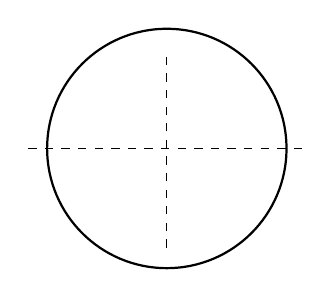
\begin{tikzpicture}
\draw[thick] (0,0) circle (1.52);
\draw[dashed] (-1.76,0)--(1.76,0);
\draw[dashed] (0,-1.26)--(0,1.26);
\end{tikzpicture}
\end{lstlisting}
\end{minipage}\hfill
\begin{minipage}{0.40\linewidth}
\centering
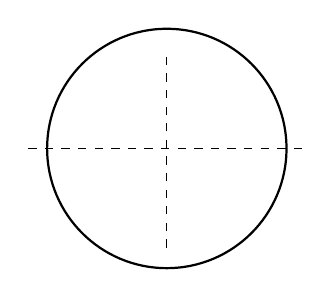
\begin{tikzpicture}
\draw[thick] (0,0) circle (1.52);
\draw[dashed] (-1.76,0)--(1.76,0);
\draw[dashed] (0,-1.26)--(0,1.26);
\end{tikzpicture}
\end{minipage}
\caption{Aylana + diametrlar (variant 16).}\label{fig:G16}
\end{figure}
\FloatBarrier
\clearpage

\subsection{G17) Geometriya chizmasi 17}
Chapda kod, o‘ngda natija. TikZ’ni odat bo‘yicha: koordinata → asosiy chiziqlar → yordamchi chiziqlar → belgilash.

\begin{figure}[H]
\centering
\begin{minipage}{0.56\linewidth}
\begin{lstlisting}
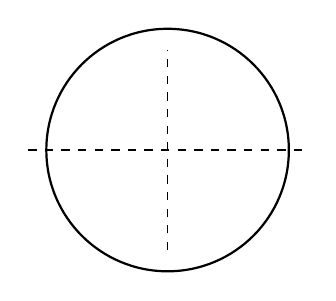
\begin{tikzpicture}
\draw[thick] (0,0) circle (1.54);
\draw[dashed] (-1.77,0)--(1.77,0);
\draw[dashed] (0,-1.27)--(0,1.27);
\end{tikzpicture}
\end{lstlisting}
\end{minipage}\hfill
\begin{minipage}{0.40\linewidth}
\centering
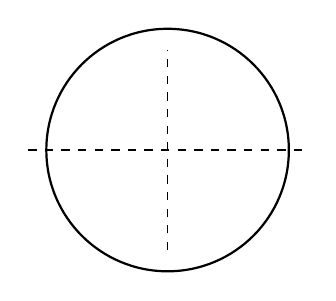
\begin{tikzpicture}
\draw[thick] (0,0) circle (1.54);
\draw[dashed] (-1.77,0)--(1.77,0);
\draw[dashed] (0,-1.27)--(0,1.27);
\end{tikzpicture}
\end{minipage}
\caption{Aylana + diametrlar (variant 17).}\label{fig:G17}
\end{figure}
\FloatBarrier
\clearpage

\subsection{G18) Geometriya chizmasi 18}
Chapda kod, o‘ngda natija. TikZ’ni odat bo‘yicha: koordinata → asosiy chiziqlar → yordamchi chiziqlar → belgilash.

\begin{figure}[H]
\centering
\begin{minipage}{0.56\linewidth}
\begin{lstlisting}
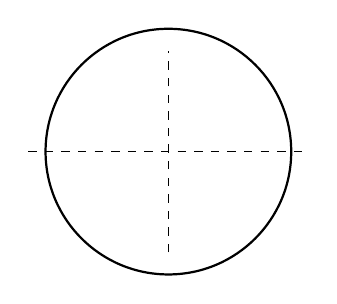
\begin{tikzpicture}
\draw[thick] (0,0) circle (1.56);
\draw[dashed] (-1.78,0)--(1.78,0);
\draw[dashed] (0,-1.28)--(0,1.28);
\end{tikzpicture}
\end{lstlisting}
\end{minipage}\hfill
\begin{minipage}{0.40\linewidth}
\centering
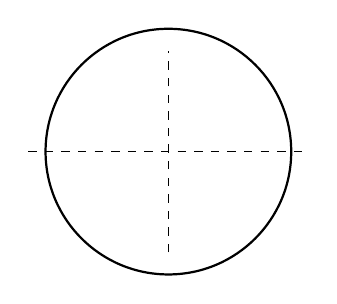
\begin{tikzpicture}
\draw[thick] (0,0) circle (1.56);
\draw[dashed] (-1.78,0)--(1.78,0);
\draw[dashed] (0,-1.28)--(0,1.28);
\end{tikzpicture}
\end{minipage}
\caption{Aylana + diametrlar (variant 18).}\label{fig:G18}
\end{figure}
\FloatBarrier
\clearpage

\subsection{G19) Geometriya chizmasi 19}
Chapda kod, o‘ngda natija. TikZ’ni odat bo‘yicha: koordinata → asosiy chiziqlar → yordamchi chiziqlar → belgilash.

\begin{figure}[H]
\centering
\begin{minipage}{0.56\linewidth}
\begin{lstlisting}
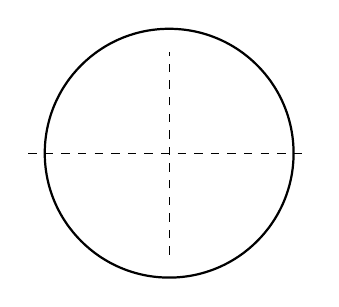
\begin{tikzpicture}
\draw[thick] (0,0) circle (1.58);
\draw[dashed] (-1.79,0)--(1.79,0);
\draw[dashed] (0,-1.29)--(0,1.29);
\end{tikzpicture}
\end{lstlisting}
\end{minipage}\hfill
\begin{minipage}{0.40\linewidth}
\centering
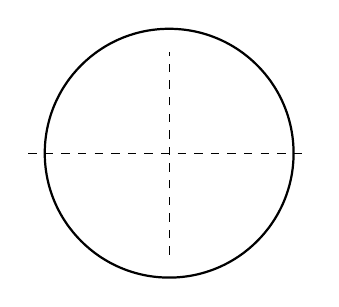
\begin{tikzpicture}
\draw[thick] (0,0) circle (1.58);
\draw[dashed] (-1.79,0)--(1.79,0);
\draw[dashed] (0,-1.29)--(0,1.29);
\end{tikzpicture}
\end{minipage}
\caption{Aylana + diametrlar (variant 19).}\label{fig:G19}
\end{figure}
\FloatBarrier
\clearpage

\subsection{G20) Geometriya chizmasi 20}
Chapda kod, o‘ngda natija. TikZ’ni odat bo‘yicha: koordinata → asosiy chiziqlar → yordamchi chiziqlar → belgilash.

\begin{figure}[H]
\centering
\begin{minipage}{0.56\linewidth}
\begin{lstlisting}
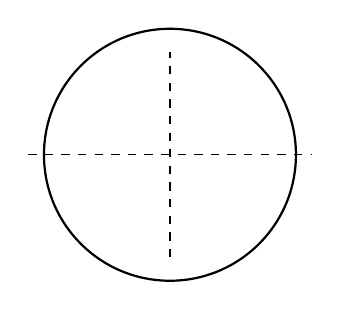
\begin{tikzpicture}
\draw[thick] (0,0) circle (1.60);
\draw[dashed] (-1.80,0)--(1.80,0);
\draw[dashed] (0,-1.30)--(0,1.30);
\end{tikzpicture}
\end{lstlisting}
\end{minipage}\hfill
\begin{minipage}{0.40\linewidth}
\centering
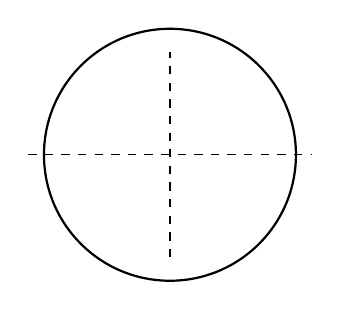
\begin{tikzpicture}
\draw[thick] (0,0) circle (1.60);
\draw[dashed] (-1.80,0)--(1.80,0);
\draw[dashed] (0,-1.30)--(0,1.30);
\end{tikzpicture}
\end{minipage}
\caption{Aylana + diametrlar (variant 20).}\label{fig:G20}
\end{figure}
\FloatBarrier
\clearpage

\subsection{G21) Geometriya chizmasi 21}
Chapda kod, o‘ngda natija. TikZ’ni odat bo‘yicha: koordinata → asosiy chiziqlar → yordamchi chiziqlar → belgilash.

\begin{figure}[H]
\centering
\begin{minipage}{0.56\linewidth}
\begin{lstlisting}
\begin{tikzpicture}
\draw[thick] (0,0) circle (1.62);
\draw[dashed] (-1.81,0)--(1.81,0);
\draw[dashed] (0,-1.31)--(0,1.31);
\end{tikzpicture}
\end{lstlisting}
\end{minipage}\hfill
\begin{minipage}{0.40\linewidth}
\centering
\begin{tikzpicture}
\draw[thick] (0,0) circle (1.62);
\draw[dashed] (-1.81,0)--(1.81,0);
\draw[dashed] (0,-1.31)--(0,1.31);
\end{tikzpicture}
\end{minipage}
\caption{Aylana + diametrlar (variant 21).}\label{fig:G21}
\end{figure}
\FloatBarrier
\clearpage

\subsection{G22) Geometriya chizmasi 22}
Chapda kod, o‘ngda natija. TikZ’ni odat bo‘yicha: koordinata → asosiy chiziqlar → yordamchi chiziqlar → belgilash.

\begin{figure}[H]
\centering
\begin{minipage}{0.56\linewidth}
\begin{lstlisting}
\begin{tikzpicture}
\draw[thick] (0,0) circle (1.64);
\draw[dashed] (-1.82,0)--(1.82,0);
\draw[dashed] (0,-1.32)--(0,1.32);
\end{tikzpicture}
\end{lstlisting}
\end{minipage}\hfill
\begin{minipage}{0.40\linewidth}
\centering
\begin{tikzpicture}
\draw[thick] (0,0) circle (1.64);
\draw[dashed] (-1.82,0)--(1.82,0);
\draw[dashed] (0,-1.32)--(0,1.32);
\end{tikzpicture}
\end{minipage}
\caption{Aylana + diametrlar (variant 22).}\label{fig:G22}
\end{figure}
\FloatBarrier
\clearpage

\subsection{G23) Geometriya chizmasi 23}
Chapda kod, o‘ngda natija. TikZ’ni odat bo‘yicha: koordinata → asosiy chiziqlar → yordamchi chiziqlar → belgilash.

\begin{figure}[H]
\centering
\begin{minipage}{0.56\linewidth}
\begin{lstlisting}
\begin{tikzpicture}
\draw[thick] (0,0) circle (1.66);
\draw[dashed] (-1.83,0)--(1.83,0);
\draw[dashed] (0,-1.33)--(0,1.33);
\end{tikzpicture}
\end{lstlisting}
\end{minipage}\hfill
\begin{minipage}{0.40\linewidth}
\centering
\begin{tikzpicture}
\draw[thick] (0,0) circle (1.66);
\draw[dashed] (-1.83,0)--(1.83,0);
\draw[dashed] (0,-1.33)--(0,1.33);
\end{tikzpicture}
\end{minipage}
\caption{Aylana + diametrlar (variant 23).}\label{fig:G23}
\end{figure}
\FloatBarrier
\clearpage

\subsection{G24) Geometriya chizmasi 24}
Chapda kod, o‘ngda natija. TikZ’ni odat bo‘yicha: koordinata → asosiy chiziqlar → yordamchi chiziqlar → belgilash.

\begin{figure}[H]
\centering
\begin{minipage}{0.56\linewidth}
\begin{lstlisting}
\begin{tikzpicture}
\draw[thick] (0,0) circle (1.68);
\draw[dashed] (-1.84,0)--(1.84,0);
\draw[dashed] (0,-1.34)--(0,1.34);
\end{tikzpicture}
\end{lstlisting}
\end{minipage}\hfill
\begin{minipage}{0.40\linewidth}
\centering
\begin{tikzpicture}
\draw[thick] (0,0) circle (1.68);
\draw[dashed] (-1.84,0)--(1.84,0);
\draw[dashed] (0,-1.34)--(0,1.34);
\end{tikzpicture}
\end{minipage}
\caption{Aylana + diametrlar (variant 24).}\label{fig:G24}
\end{figure}
\FloatBarrier
\clearpage

\subsection{G25) Geometriya chizmasi 25}
Chapda kod, o‘ngda natija. TikZ’ni odat bo‘yicha: koordinata → asosiy chiziqlar → yordamchi chiziqlar → belgilash.

\begin{figure}[H]
\centering
\begin{minipage}{0.56\linewidth}
\begin{lstlisting}
\begin{tikzpicture}
\draw[thick] (0,0) circle (1.70);
\draw[dashed] (-1.85,0)--(1.85,0);
\draw[dashed] (0,-1.35)--(0,1.35);
\end{tikzpicture}
\end{lstlisting}
\end{minipage}\hfill
\begin{minipage}{0.40\linewidth}
\centering
\begin{tikzpicture}
\draw[thick] (0,0) circle (1.70);
\draw[dashed] (-1.85,0)--(1.85,0);
\draw[dashed] (0,-1.35)--(0,1.35);
\end{tikzpicture}
\end{minipage}
\caption{Aylana + diametrlar (variant 25).}\label{fig:G25}
\end{figure}
\FloatBarrier
\clearpage

\subsection{G26) Geometriya chizmasi 26}
Chapda kod, o‘ngda natija. TikZ’ni odat bo‘yicha: koordinata → asosiy chiziqlar → yordamchi chiziqlar → belgilash.

\begin{figure}[H]
\centering
\begin{minipage}{0.56\linewidth}
\begin{lstlisting}
\begin{tikzpicture}
\draw[thick] (0,0) circle (1.72);
\draw[dashed] (-1.86,0)--(1.86,0);
\draw[dashed] (0,-1.36)--(0,1.36);
\end{tikzpicture}
\end{lstlisting}
\end{minipage}\hfill
\begin{minipage}{0.40\linewidth}
\centering
\begin{tikzpicture}
\draw[thick] (0,0) circle (1.72);
\draw[dashed] (-1.86,0)--(1.86,0);
\draw[dashed] (0,-1.36)--(0,1.36);
\end{tikzpicture}
\end{minipage}
\caption{Aylana + diametrlar (variant 26).}\label{fig:G26}
\end{figure}
\FloatBarrier
\clearpage

\subsection{G27) Geometriya chizmasi 27}
Chapda kod, o‘ngda natija. TikZ’ni odat bo‘yicha: koordinata → asosiy chiziqlar → yordamchi chiziqlar → belgilash.

\begin{figure}[H]
\centering
\begin{minipage}{0.56\linewidth}
\begin{lstlisting}
\begin{tikzpicture}
\draw[thick] (0,0) circle (1.74);
\draw[dashed] (-1.87,0)--(1.87,0);
\draw[dashed] (0,-1.37)--(0,1.37);
\end{tikzpicture}
\end{lstlisting}
\end{minipage}\hfill
\begin{minipage}{0.40\linewidth}
\centering
\begin{tikzpicture}
\draw[thick] (0,0) circle (1.74);
\draw[dashed] (-1.87,0)--(1.87,0);
\draw[dashed] (0,-1.37)--(0,1.37);
\end{tikzpicture}
\end{minipage}
\caption{Aylana + diametrlar (variant 27).}\label{fig:G27}
\end{figure}
\FloatBarrier
\clearpage

\subsection{G28) Geometriya chizmasi 28}
Chapda kod, o‘ngda natija. TikZ’ni odat bo‘yicha: koordinata → asosiy chiziqlar → yordamchi chiziqlar → belgilash.

\begin{figure}[H]
\centering
\begin{minipage}{0.56\linewidth}
\begin{lstlisting}
\begin{tikzpicture}
\draw[thick] (0,0) circle (1.76);
\draw[dashed] (-1.88,0)--(1.88,0);
\draw[dashed] (0,-1.38)--(0,1.38);
\end{tikzpicture}
\end{lstlisting}
\end{minipage}\hfill
\begin{minipage}{0.40\linewidth}
\centering
\begin{tikzpicture}
\draw[thick] (0,0) circle (1.76);
\draw[dashed] (-1.88,0)--(1.88,0);
\draw[dashed] (0,-1.38)--(0,1.38);
\end{tikzpicture}
\end{minipage}
\caption{Aylana + diametrlar (variant 28).}\label{fig:G28}
\end{figure}
\FloatBarrier
\clearpage

\subsection{G29) Geometriya chizmasi 29}
Chapda kod, o‘ngda natija. TikZ’ni odat bo‘yicha: koordinata → asosiy chiziqlar → yordamchi chiziqlar → belgilash.

\begin{figure}[H]
\centering
\begin{minipage}{0.56\linewidth}
\begin{lstlisting}
\begin{tikzpicture}
\draw[thick] (0,0) circle (1.78);
\draw[dashed] (-1.89,0)--(1.89,0);
\draw[dashed] (0,-1.39)--(0,1.39);
\end{tikzpicture}
\end{lstlisting}
\end{minipage}\hfill
\begin{minipage}{0.40\linewidth}
\centering
\begin{tikzpicture}
\draw[thick] (0,0) circle (1.78);
\draw[dashed] (-1.89,0)--(1.89,0);
\draw[dashed] (0,-1.39)--(0,1.39);
\end{tikzpicture}
\end{minipage}
\caption{Aylana + diametrlar (variant 29).}\label{fig:G29}
\end{figure}
\FloatBarrier
\clearpage

\subsection{G30) Geometriya chizmasi 30}
Chapda kod, o‘ngda natija. TikZ’ni odat bo‘yicha: koordinata → asosiy chiziqlar → yordamchi chiziqlar → belgilash.

\begin{figure}[H]
\centering
\begin{minipage}{0.56\linewidth}
\begin{lstlisting}
\begin{tikzpicture}
\draw[thick] (0,0) circle (1.80);
\draw[dashed] (-1.90,0)--(1.90,0);
\draw[dashed] (0,-1.40)--(0,1.40);
\end{tikzpicture}
\end{lstlisting}
\end{minipage}\hfill
\begin{minipage}{0.40\linewidth}
\centering
\begin{tikzpicture}
\draw[thick] (0,0) circle (1.80);
\draw[dashed] (-1.90,0)--(1.90,0);
\draw[dashed] (0,-1.40)--(0,1.40);
\end{tikzpicture}
\end{minipage}
\caption{Aylana + diametrlar (variant 30).}\label{fig:G30}
\end{figure}
\FloatBarrier
\clearpage

\subsection{O1) Olimpiada diagrammasi 1}
Skelet usuli: avval kontur, keyin yordamchi chiziqlar, oxiri label/nuqtalar.

\begin{figure}[H]
\centering
\begin{minipage}{0.56\linewidth}
\begin{lstlisting}
\begin{tikzpicture}
\coordinate (A) at (0,0);\coordinate (B) at (5,0);\coordinate (C) at (1.6,3.2);
\draw[thick] (A)--(B)--(C)--cycle;
\coordinate (D) at ($(B)!0.35!(C)$);
\coordinate (E) at ($(C)!0.55!(A)$);
\path[name path=AD] (A)--(D);
\path[name path=BE] (B)--(E);
\draw[dashed] (A)--(D);
\draw[dashed] (B)--(E);
\path[name intersections={of=AD and BE, by=P}];
\fill (P) circle(1.5pt);
\end{tikzpicture}
\end{lstlisting}
\end{minipage}\hfill
\begin{minipage}{0.40\linewidth}
\centering
\begin{tikzpicture}
\coordinate (A) at (0,0);\coordinate (B) at (5,0);\coordinate (C) at (1.6,3.2);
\draw[thick] (A)--(B)--(C)--cycle;
\coordinate (D) at ($(B)!0.35!(C)$);
\coordinate (E) at ($(C)!0.55!(A)$);
\path[name path=AD] (A)--(D);
\path[name path=BE] (B)--(E);
\draw[dashed] (A)--(D);
\draw[dashed] (B)--(E);
\path[name intersections={of=AD and BE, by=P}];
\fill (P) circle(1.5pt);
\end{tikzpicture}
\end{minipage}
\caption{Ceva skeleti: cevians kesishmasi.}\label{fig:O1}
\end{figure}
\FloatBarrier
\clearpage

\subsection{O2) Olimpiada diagrammasi 2}
Skelet usuli: avval kontur, keyin yordamchi chiziqlar, oxiri label/nuqtalar.

\begin{figure}[H]
\centering
\begin{minipage}{0.56\linewidth}
\begin{lstlisting}
\begin{tikzpicture}
\coordinate (O) at (0,0);
\draw[thick] (O) circle (2.2);
\coordinate (A) at (140:2.2);
\coordinate (B) at (20:2.2);
\coordinate (C) at (-70:2.2);
\draw[thick] (A)--(B)--(C)--cycle;
\coordinate (P) at (250:2.2);
\coordinate (Ha) at ($(B)!(P)!(C)$);
\coordinate (Hb) at ($(C)!(P)!(A)$);
\coordinate (Hc) at ($(A)!(P)!(B)$);
\draw[dashed] (Ha)--(Hb)--(Hc);
\end{tikzpicture}
\end{lstlisting}
\end{minipage}\hfill
\begin{minipage}{0.40\linewidth}
\centering
\begin{tikzpicture}
\coordinate (O) at (0,0);
\draw[thick] (O) circle (2.2);
\coordinate (A) at (140:2.2);
\coordinate (B) at (20:2.2);
\coordinate (C) at (-70:2.2);
\draw[thick] (A)--(B)--(C)--cycle;
\coordinate (P) at (250:2.2);
\coordinate (Ha) at ($(B)!(P)!(C)$);
\coordinate (Hb) at ($(C)!(P)!(A)$);
\coordinate (Hc) at ($(A)!(P)!(B)$);
\draw[dashed] (Ha)--(Hb)--(Hc);
\end{tikzpicture}
\end{minipage}
\caption{Simson line (schematic): 3 proyeksiya oyoği.}\label{fig:O2}
\end{figure}
\FloatBarrier
\clearpage

\subsection{O3) Olimpiada diagrammasi 3}
Skelet usuli: avval kontur, keyin yordamchi chiziqlar, oxiri label/nuqtalar.

\begin{figure}[H]
\centering
\begin{minipage}{0.56\linewidth}
\begin{lstlisting}
\begin{tikzpicture}
\draw[thick] (0,0) ellipse (2.26 and 1.43);
\foreach \ang in {150,90,30,-20,-80,-140} {\fill (\ang:2.26) circle(1.1pt);}
\draw[dashed] (-3.0,-0.7) -- (3.0,0.9);
\end{tikzpicture}
\end{lstlisting}
\end{minipage}\hfill
\begin{minipage}{0.40\linewidth}
\centering
\begin{tikzpicture}
\draw[thick] (0,0) ellipse (2.26 and 1.43);
\foreach \ang in {150,90,30,-20,-80,-140} {\fill (\ang:2.26) circle(1.1pt);}
\draw[dashed] (-3.0,-0.7) -- (3.0,0.9);
\end{tikzpicture}
\end{minipage}
\caption{Olimpiada skeleti (variant 3): konik + transversal.}\label{fig:O3}
\end{figure}
\FloatBarrier
\clearpage

\subsection{O4) Olimpiada diagrammasi 4}
Skelet usuli: avval kontur, keyin yordamchi chiziqlar, oxiri label/nuqtalar.

\begin{figure}[H]
\centering
\begin{minipage}{0.56\linewidth}
\begin{lstlisting}
\begin{tikzpicture}
\draw[thick] (0,0) ellipse (2.28 and 1.44);
\foreach \ang in {150,90,30,-20,-80,-140} {\fill (\ang:2.28) circle(1.1pt);}
\draw[dashed] (-3.0,-0.7) -- (3.0,0.9);
\end{tikzpicture}
\end{lstlisting}
\end{minipage}\hfill
\begin{minipage}{0.40\linewidth}
\centering
\begin{tikzpicture}
\draw[thick] (0,0) ellipse (2.28 and 1.44);
\foreach \ang in {150,90,30,-20,-80,-140} {\fill (\ang:2.28) circle(1.1pt);}
\draw[dashed] (-3.0,-0.7) -- (3.0,0.9);
\end{tikzpicture}
\end{minipage}
\caption{Olimpiada skeleti (variant 4): konik + transversal.}\label{fig:O4}
\end{figure}
\FloatBarrier
\clearpage

\subsection{O5) Olimpiada diagrammasi 5}
Skelet usuli: avval kontur, keyin yordamchi chiziqlar, oxiri label/nuqtalar.

\begin{figure}[H]
\centering
\begin{minipage}{0.56\linewidth}
\begin{lstlisting}
\begin{tikzpicture}
\draw[thick] (0,0) ellipse (2.30 and 1.45);
\foreach \ang in {150,90,30,-20,-80,-140} {\fill (\ang:2.30) circle(1.1pt);}
\draw[dashed] (-3.0,-0.7) -- (3.0,0.9);
\end{tikzpicture}
\end{lstlisting}
\end{minipage}\hfill
\begin{minipage}{0.40\linewidth}
\centering
\begin{tikzpicture}
\draw[thick] (0,0) ellipse (2.30 and 1.45);
\foreach \ang in {150,90,30,-20,-80,-140} {\fill (\ang:2.30) circle(1.1pt);}
\draw[dashed] (-3.0,-0.7) -- (3.0,0.9);
\end{tikzpicture}
\end{minipage}
\caption{Olimpiada skeleti (variant 5): konik + transversal.}\label{fig:O5}
\end{figure}
\FloatBarrier
\clearpage

\subsection{O6) Olimpiada diagrammasi 6}
Skelet usuli: avval kontur, keyin yordamchi chiziqlar, oxiri label/nuqtalar.

\begin{figure}[H]
\centering
\begin{minipage}{0.56\linewidth}
\begin{lstlisting}
\begin{tikzpicture}
\draw[thick] (0,0) ellipse (2.32 and 1.46);
\foreach \ang in {150,90,30,-20,-80,-140} {\fill (\ang:2.32) circle(1.1pt);}
\draw[dashed] (-3.0,-0.7) -- (3.0,0.9);
\end{tikzpicture}
\end{lstlisting}
\end{minipage}\hfill
\begin{minipage}{0.40\linewidth}
\centering
\begin{tikzpicture}
\draw[thick] (0,0) ellipse (2.32 and 1.46);
\foreach \ang in {150,90,30,-20,-80,-140} {\fill (\ang:2.32) circle(1.1pt);}
\draw[dashed] (-3.0,-0.7) -- (3.0,0.9);
\end{tikzpicture}
\end{minipage}
\caption{Olimpiada skeleti (variant 6): konik + transversal.}\label{fig:O6}
\end{figure}
\FloatBarrier
\clearpage

\subsection{O7) Olimpiada diagrammasi 7}
Skelet usuli: avval kontur, keyin yordamchi chiziqlar, oxiri label/nuqtalar.

\begin{figure}[H]
\centering
\begin{minipage}{0.56\linewidth}
\begin{lstlisting}
\begin{tikzpicture}
\draw[thick] (0,0) ellipse (2.34 and 1.47);
\foreach \ang in {150,90,30,-20,-80,-140} {\fill (\ang:2.34) circle(1.1pt);}
\draw[dashed] (-3.0,-0.7) -- (3.0,0.9);
\end{tikzpicture}
\end{lstlisting}
\end{minipage}\hfill
\begin{minipage}{0.40\linewidth}
\centering
\begin{tikzpicture}
\draw[thick] (0,0) ellipse (2.34 and 1.47);
\foreach \ang in {150,90,30,-20,-80,-140} {\fill (\ang:2.34) circle(1.1pt);}
\draw[dashed] (-3.0,-0.7) -- (3.0,0.9);
\end{tikzpicture}
\end{minipage}
\caption{Olimpiada skeleti (variant 7): konik + transversal.}\label{fig:O7}
\end{figure}
\FloatBarrier
\clearpage

\subsection{O8) Olimpiada diagrammasi 8}
Skelet usuli: avval kontur, keyin yordamchi chiziqlar, oxiri label/nuqtalar.

\begin{figure}[H]
\centering
\begin{minipage}{0.56\linewidth}
\begin{lstlisting}
\begin{tikzpicture}
\draw[thick] (0,0) ellipse (2.36 and 1.48);
\foreach \ang in {150,90,30,-20,-80,-140} {\fill (\ang:2.36) circle(1.1pt);}
\draw[dashed] (-3.0,-0.7) -- (3.0,0.9);
\end{tikzpicture}
\end{lstlisting}
\end{minipage}\hfill
\begin{minipage}{0.40\linewidth}
\centering
\begin{tikzpicture}
\draw[thick] (0,0) ellipse (2.36 and 1.48);
\foreach \ang in {150,90,30,-20,-80,-140} {\fill (\ang:2.36) circle(1.1pt);}
\draw[dashed] (-3.0,-0.7) -- (3.0,0.9);
\end{tikzpicture}
\end{minipage}
\caption{Olimpiada skeleti (variant 8): konik + transversal.}\label{fig:O8}
\end{figure}
\FloatBarrier
\clearpage

\subsection{O9) Olimpiada diagrammasi 9}
Skelet usuli: avval kontur, keyin yordamchi chiziqlar, oxiri label/nuqtalar.

\begin{figure}[H]
\centering
\begin{minipage}{0.56\linewidth}
\begin{lstlisting}
\begin{tikzpicture}
\draw[thick] (0,0) ellipse (2.38 and 1.49);
\foreach \ang in {150,90,30,-20,-80,-140} {\fill (\ang:2.38) circle(1.1pt);}
\draw[dashed] (-3.0,-0.7) -- (3.0,0.9);
\end{tikzpicture}
\end{lstlisting}
\end{minipage}\hfill
\begin{minipage}{0.40\linewidth}
\centering
\begin{tikzpicture}
\draw[thick] (0,0) ellipse (2.38 and 1.49);
\foreach \ang in {150,90,30,-20,-80,-140} {\fill (\ang:2.38) circle(1.1pt);}
\draw[dashed] (-3.0,-0.7) -- (3.0,0.9);
\end{tikzpicture}
\end{minipage}
\caption{Olimpiada skeleti (variant 9): konik + transversal.}\label{fig:O9}
\end{figure}
\FloatBarrier
\clearpage

\subsection{O10) Olimpiada diagrammasi 10}
Skelet usuli: avval kontur, keyin yordamchi chiziqlar, oxiri label/nuqtalar.

\begin{figure}[H]
\centering
\begin{minipage}{0.56\linewidth}
\begin{lstlisting}
\begin{tikzpicture}
\draw[thick] (0,0) ellipse (2.40 and 1.50);
\foreach \ang in {150,90,30,-20,-80,-140} {\fill (\ang:2.40) circle(1.1pt);}
\draw[dashed] (-3.0,-0.7) -- (3.0,0.9);
\end{tikzpicture}
\end{lstlisting}
\end{minipage}\hfill
\begin{minipage}{0.40\linewidth}
\centering
\begin{tikzpicture}
\draw[thick] (0,0) ellipse (2.40 and 1.50);
\foreach \ang in {150,90,30,-20,-80,-140} {\fill (\ang:2.40) circle(1.1pt);}
\draw[dashed] (-3.0,-0.7) -- (3.0,0.9);
\end{tikzpicture}
\end{minipage}
\caption{Olimpiada skeleti (variant 10): konik + transversal.}\label{fig:O10}
\end{figure}
\FloatBarrier
\clearpage

\subsection{O11) Olimpiada diagrammasi 11}
Skelet usuli: avval kontur, keyin yordamchi chiziqlar, oxiri label/nuqtalar.

\begin{figure}[H]
\centering
\begin{minipage}{0.56\linewidth}
\begin{lstlisting}
\begin{tikzpicture}
\draw[thick] (0,0) ellipse (2.42 and 1.51);
\foreach \ang in {150,90,30,-20,-80,-140} {\fill (\ang:2.42) circle(1.1pt);}
\draw[dashed] (-3.0,-0.7) -- (3.0,0.9);
\end{tikzpicture}
\end{lstlisting}
\end{minipage}\hfill
\begin{minipage}{0.40\linewidth}
\centering
\begin{tikzpicture}
\draw[thick] (0,0) ellipse (2.42 and 1.51);
\foreach \ang in {150,90,30,-20,-80,-140} {\fill (\ang:2.42) circle(1.1pt);}
\draw[dashed] (-3.0,-0.7) -- (3.0,0.9);
\end{tikzpicture}
\end{minipage}
\caption{Olimpiada skeleti (variant 11): konik + transversal.}\label{fig:O11}
\end{figure}
\FloatBarrier
\clearpage

\subsection{O12) Olimpiada diagrammasi 12}
Skelet usuli: avval kontur, keyin yordamchi chiziqlar, oxiri label/nuqtalar.

\begin{figure}[H]
\centering
\begin{minipage}{0.56\linewidth}
\begin{lstlisting}
\begin{tikzpicture}
\draw[thick] (0,0) ellipse (2.44 and 1.52);
\foreach \ang in {150,90,30,-20,-80,-140} {\fill (\ang:2.44) circle(1.1pt);}
\draw[dashed] (-3.0,-0.7) -- (3.0,0.9);
\end{tikzpicture}
\end{lstlisting}
\end{minipage}\hfill
\begin{minipage}{0.40\linewidth}
\centering
\begin{tikzpicture}
\draw[thick] (0,0) ellipse (2.44 and 1.52);
\foreach \ang in {150,90,30,-20,-80,-140} {\fill (\ang:2.44) circle(1.1pt);}
\draw[dashed] (-3.0,-0.7) -- (3.0,0.9);
\end{tikzpicture}
\end{minipage}
\caption{Olimpiada skeleti (variant 12): konik + transversal.}\label{fig:O12}
\end{figure}
\FloatBarrier
\clearpage

\subsection{O13) Olimpiada diagrammasi 13}
Skelet usuli: avval kontur, keyin yordamchi chiziqlar, oxiri label/nuqtalar.

\begin{figure}[H]
\centering
\begin{minipage}{0.56\linewidth}
\begin{lstlisting}
\begin{tikzpicture}
\draw[thick] (0,0) ellipse (2.46 and 1.53);
\foreach \ang in {150,90,30,-20,-80,-140} {\fill (\ang:2.46) circle(1.1pt);}
\draw[dashed] (-3.0,-0.7) -- (3.0,0.9);
\end{tikzpicture}
\end{lstlisting}
\end{minipage}\hfill
\begin{minipage}{0.40\linewidth}
\centering
\begin{tikzpicture}
\draw[thick] (0,0) ellipse (2.46 and 1.53);
\foreach \ang in {150,90,30,-20,-80,-140} {\fill (\ang:2.46) circle(1.1pt);}
\draw[dashed] (-3.0,-0.7) -- (3.0,0.9);
\end{tikzpicture}
\end{minipage}
\caption{Olimpiada skeleti (variant 13): konik + transversal.}\label{fig:O13}
\end{figure}
\FloatBarrier
\clearpage

\subsection{O14) Olimpiada diagrammasi 14}
Skelet usuli: avval kontur, keyin yordamchi chiziqlar, oxiri label/nuqtalar.

\begin{figure}[H]
\centering
\begin{minipage}{0.56\linewidth}
\begin{lstlisting}
\begin{tikzpicture}
\draw[thick] (0,0) ellipse (2.48 and 1.54);
\foreach \ang in {150,90,30,-20,-80,-140} {\fill (\ang:2.48) circle(1.1pt);}
\draw[dashed] (-3.0,-0.7) -- (3.0,0.9);
\end{tikzpicture}
\end{lstlisting}
\end{minipage}\hfill
\begin{minipage}{0.40\linewidth}
\centering
\begin{tikzpicture}
\draw[thick] (0,0) ellipse (2.48 and 1.54);
\foreach \ang in {150,90,30,-20,-80,-140} {\fill (\ang:2.48) circle(1.1pt);}
\draw[dashed] (-3.0,-0.7) -- (3.0,0.9);
\end{tikzpicture}
\end{minipage}
\caption{Olimpiada skeleti (variant 14): konik + transversal.}\label{fig:O14}
\end{figure}
\FloatBarrier
\clearpage

\subsection{O15) Olimpiada diagrammasi 15}
Skelet usuli: avval kontur, keyin yordamchi chiziqlar, oxiri label/nuqtalar.

\begin{figure}[H]
\centering
\begin{minipage}{0.56\linewidth}
\begin{lstlisting}
\begin{tikzpicture}
\draw[thick] (0,0) ellipse (2.50 and 1.55);
\foreach \ang in {150,90,30,-20,-80,-140} {\fill (\ang:2.50) circle(1.1pt);}
\draw[dashed] (-3.0,-0.7) -- (3.0,0.9);
\end{tikzpicture}
\end{lstlisting}
\end{minipage}\hfill
\begin{minipage}{0.40\linewidth}
\centering
\begin{tikzpicture}
\draw[thick] (0,0) ellipse (2.50 and 1.55);
\foreach \ang in {150,90,30,-20,-80,-140} {\fill (\ang:2.50) circle(1.1pt);}
\draw[dashed] (-3.0,-0.7) -- (3.0,0.9);
\end{tikzpicture}
\end{minipage}
\caption{Olimpiada skeleti (variant 15): konik + transversal.}\label{fig:O15}
\end{figure}
\FloatBarrier
\clearpage

\subsection{O16) Olimpiada diagrammasi 16}
Skelet usuli: avval kontur, keyin yordamchi chiziqlar, oxiri label/nuqtalar.

\begin{figure}[H]
\centering
\begin{minipage}{0.56\linewidth}
\begin{lstlisting}
\begin{tikzpicture}
\draw[thick] (0,0) ellipse (2.52 and 1.56);
\foreach \ang in {150,90,30,-20,-80,-140} {\fill (\ang:2.52) circle(1.1pt);}
\draw[dashed] (-3.0,-0.7) -- (3.0,0.9);
\end{tikzpicture}
\end{lstlisting}
\end{minipage}\hfill
\begin{minipage}{0.40\linewidth}
\centering
\begin{tikzpicture}
\draw[thick] (0,0) ellipse (2.52 and 1.56);
\foreach \ang in {150,90,30,-20,-80,-140} {\fill (\ang:2.52) circle(1.1pt);}
\draw[dashed] (-3.0,-0.7) -- (3.0,0.9);
\end{tikzpicture}
\end{minipage}
\caption{Olimpiada skeleti (variant 16): konik + transversal.}\label{fig:O16}
\end{figure}
\FloatBarrier
\clearpage

\subsection{O17) Olimpiada diagrammasi 17}
Skelet usuli: avval kontur, keyin yordamchi chiziqlar, oxiri label/nuqtalar.

\begin{figure}[H]
\centering
\begin{minipage}{0.56\linewidth}
\begin{lstlisting}
\begin{tikzpicture}
\draw[thick] (0,0) ellipse (2.54 and 1.57);
\foreach \ang in {150,90,30,-20,-80,-140} {\fill (\ang:2.54) circle(1.1pt);}
\draw[dashed] (-3.0,-0.7) -- (3.0,0.9);
\end{tikzpicture}
\end{lstlisting}
\end{minipage}\hfill
\begin{minipage}{0.40\linewidth}
\centering
\begin{tikzpicture}
\draw[thick] (0,0) ellipse (2.54 and 1.57);
\foreach \ang in {150,90,30,-20,-80,-140} {\fill (\ang:2.54) circle(1.1pt);}
\draw[dashed] (-3.0,-0.7) -- (3.0,0.9);
\end{tikzpicture}
\end{minipage}
\caption{Olimpiada skeleti (variant 17): konik + transversal.}\label{fig:O17}
\end{figure}
\FloatBarrier
\clearpage

\subsection{O18) Olimpiada diagrammasi 18}
Skelet usuli: avval kontur, keyin yordamchi chiziqlar, oxiri label/nuqtalar.

\begin{figure}[H]
\centering
\begin{minipage}{0.56\linewidth}
\begin{lstlisting}
\begin{tikzpicture}
\draw[thick] (0,0) ellipse (2.56 and 1.58);
\foreach \ang in {150,90,30,-20,-80,-140} {\fill (\ang:2.56) circle(1.1pt);}
\draw[dashed] (-3.0,-0.7) -- (3.0,0.9);
\end{tikzpicture}
\end{lstlisting}
\end{minipage}\hfill
\begin{minipage}{0.40\linewidth}
\centering
\begin{tikzpicture}
\draw[thick] (0,0) ellipse (2.56 and 1.58);
\foreach \ang in {150,90,30,-20,-80,-140} {\fill (\ang:2.56) circle(1.1pt);}
\draw[dashed] (-3.0,-0.7) -- (3.0,0.9);
\end{tikzpicture}
\end{minipage}
\caption{Olimpiada skeleti (variant 18): konik + transversal.}\label{fig:O18}
\end{figure}
\FloatBarrier
\clearpage

\subsection{O19) Olimpiada diagrammasi 19}
Skelet usuli: avval kontur, keyin yordamchi chiziqlar, oxiri label/nuqtalar.

\begin{figure}[H]
\centering
\begin{minipage}{0.56\linewidth}
\begin{lstlisting}
\begin{tikzpicture}
\draw[thick] (0,0) ellipse (2.58 and 1.59);
\foreach \ang in {150,90,30,-20,-80,-140} {\fill (\ang:2.58) circle(1.1pt);}
\draw[dashed] (-3.0,-0.7) -- (3.0,0.9);
\end{tikzpicture}
\end{lstlisting}
\end{minipage}\hfill
\begin{minipage}{0.40\linewidth}
\centering
\begin{tikzpicture}
\draw[thick] (0,0) ellipse (2.58 and 1.59);
\foreach \ang in {150,90,30,-20,-80,-140} {\fill (\ang:2.58) circle(1.1pt);}
\draw[dashed] (-3.0,-0.7) -- (3.0,0.9);
\end{tikzpicture}
\end{minipage}
\caption{Olimpiada skeleti (variant 19): konik + transversal.}\label{fig:O19}
\end{figure}
\FloatBarrier
\clearpage

\subsection{O20) Olimpiada diagrammasi 20}
Skelet usuli: avval kontur, keyin yordamchi chiziqlar, oxiri label/nuqtalar.

\begin{figure}[H]
\centering
\begin{minipage}{0.56\linewidth}
\begin{lstlisting}
\begin{tikzpicture}
\draw[thick] (0,0) ellipse (2.60 and 1.60);
\foreach \ang in {150,90,30,-20,-80,-140} {\fill (\ang:2.60) circle(1.1pt);}
\draw[dashed] (-3.0,-0.7) -- (3.0,0.9);
\end{tikzpicture}
\end{lstlisting}
\end{minipage}\hfill
\begin{minipage}{0.40\linewidth}
\centering
\begin{tikzpicture}
\draw[thick] (0,0) ellipse (2.60 and 1.60);
\foreach \ang in {150,90,30,-20,-80,-140} {\fill (\ang:2.60) circle(1.1pt);}
\draw[dashed] (-3.0,-0.7) -- (3.0,0.9);
\end{tikzpicture}
\end{minipage}
\caption{Olimpiada skeleti (variant 20): konik + transversal.}\label{fig:O20}
\end{figure}
\FloatBarrier
\clearpage

\subsection{P1) PGFPlots grafigi 1}
PGFPlots’da: axis sozlamalari (o‘q/label/grid) → addplot → legenda.

\begin{figure}[H]
\centering
\begin{minipage}{0.56\linewidth}
\begin{lstlisting}
\begin{tikzpicture}
\begin{axis}[width=0.95\linewidth, xlabel={$x$}, ylabel={$x^2$}, grid=both]
\addplot[domain=-2:2, samples=200]{x^2};
\end{axis}
\end{tikzpicture}
\end{lstlisting}
\end{minipage}\hfill
\begin{minipage}{0.40\linewidth}
\centering
\begin{tikzpicture}
\begin{axis}[width=0.95\linewidth, xlabel={$x$}, ylabel={$x^2$}, grid=both]
\addplot[domain=-2:2, samples=200]{x^2};
\end{axis}
\end{tikzpicture}
\end{minipage}
\caption{PGFPlots: $y=x^2$.}\label{fig:P1}
\end{figure}
\FloatBarrier
\clearpage

\subsection{P2) PGFPlots grafigi 2}
PGFPlots’da: axis sozlamalari (o‘q/label/grid) → addplot → legenda.

\begin{figure}[H]
\centering
\begin{minipage}{0.56\linewidth}
\begin{lstlisting}
\begin{tikzpicture}
\begin{axis}[width=0.95\linewidth, xlabel={$x$}, ylabel={$f(x)$}, grid=both, legend pos=north west]
\addplot[domain=0:6.28, samples=300]{sin(deg(2*x))};
\addlegendentry{$\sin(2x)$}
\end{axis}
\end{tikzpicture}
\end{lstlisting}
\end{minipage}\hfill
\begin{minipage}{0.40\linewidth}
\centering
\begin{tikzpicture}
\begin{axis}[width=0.95\linewidth, xlabel={$x$}, ylabel={$f(x)$}, grid=both, legend pos=north west]
\addplot[domain=0:6.28, samples=300]{sin(deg(2*x))};
\addlegendentry{$\sin(2x)$}
\end{axis}
\end{tikzpicture}
\end{minipage}
\caption{PGFPlots: $\sin(2x)$.}\label{fig:P2}
\end{figure}
\FloatBarrier
\clearpage

\subsection{P3) PGFPlots grafigi 3}
PGFPlots’da: axis sozlamalari (o‘q/label/grid) → addplot → legenda.

\begin{figure}[H]
\centering
\begin{minipage}{0.56\linewidth}
\begin{lstlisting}
\begin{tikzpicture}
\begin{axis}[width=0.95\linewidth, xlabel={$x$}, ylabel={$f(x)$}, grid=both, legend pos=north west]
\addplot[domain=0:6.28, samples=300]{sin(deg(3*x))};
\addlegendentry{$\sin(3x)$}
\end{axis}
\end{tikzpicture}
\end{lstlisting}
\end{minipage}\hfill
\begin{minipage}{0.40\linewidth}
\centering
\begin{tikzpicture}
\begin{axis}[width=0.95\linewidth, xlabel={$x$}, ylabel={$f(x)$}, grid=both, legend pos=north west]
\addplot[domain=0:6.28, samples=300]{sin(deg(3*x))};
\addlegendentry{$\sin(3x)$}
\end{axis}
\end{tikzpicture}
\end{minipage}
\caption{PGFPlots: $\sin(3x)$.}\label{fig:P3}
\end{figure}
\FloatBarrier
\clearpage

\subsection{P4) PGFPlots grafigi 4}
PGFPlots’da: axis sozlamalari (o‘q/label/grid) → addplot → legenda.

\begin{figure}[H]
\centering
\begin{minipage}{0.56\linewidth}
\begin{lstlisting}
\begin{tikzpicture}
\begin{axis}[width=0.95\linewidth, xlabel={$x$}, ylabel={$f(x)$}, grid=both, legend pos=north west]
\addplot[domain=0:6.28, samples=300]{sin(deg(4*x))};
\addlegendentry{$\sin(4x)$}
\end{axis}
\end{tikzpicture}
\end{lstlisting}
\end{minipage}\hfill
\begin{minipage}{0.40\linewidth}
\centering
\begin{tikzpicture}
\begin{axis}[width=0.95\linewidth, xlabel={$x$}, ylabel={$f(x)$}, grid=both, legend pos=north west]
\addplot[domain=0:6.28, samples=300]{sin(deg(4*x))};
\addlegendentry{$\sin(4x)$}
\end{axis}
\end{tikzpicture}
\end{minipage}
\caption{PGFPlots: $\sin(4x)$.}\label{fig:P4}
\end{figure}
\FloatBarrier
\clearpage

\subsection{P5) PGFPlots grafigi 5}
PGFPlots’da: axis sozlamalari (o‘q/label/grid) → addplot → legenda.

\begin{figure}[H]
\centering
\begin{minipage}{0.56\linewidth}
\begin{lstlisting}
\begin{tikzpicture}
\begin{axis}[width=0.95\linewidth, xlabel={$x$}, ylabel={$f(x)$}, grid=both, legend pos=north west]
\addplot[domain=0:6.28, samples=300]{sin(deg(5*x))};
\addlegendentry{$\sin(5x)$}
\end{axis}
\end{tikzpicture}
\end{lstlisting}
\end{minipage}\hfill
\begin{minipage}{0.40\linewidth}
\centering
\begin{tikzpicture}
\begin{axis}[width=0.95\linewidth, xlabel={$x$}, ylabel={$f(x)$}, grid=both, legend pos=north west]
\addplot[domain=0:6.28, samples=300]{sin(deg(5*x))};
\addlegendentry{$\sin(5x)$}
\end{axis}
\end{tikzpicture}
\end{minipage}
\caption{PGFPlots: $\sin(5x)$.}\label{fig:P5}
\end{figure}
\FloatBarrier
\clearpage

\subsection{P6) PGFPlots grafigi 6}
PGFPlots’da: axis sozlamalari (o‘q/label/grid) → addplot → legenda.

\begin{figure}[H]
\centering
\begin{minipage}{0.56\linewidth}
\begin{lstlisting}
\begin{tikzpicture}
\begin{axis}[width=0.95\linewidth, xlabel={$x$}, ylabel={$f(x)$}, grid=both, legend pos=north west]
\addplot[domain=0:6.28, samples=300]{sin(deg(6*x))};
\addlegendentry{$\sin(6x)$}
\end{axis}
\end{tikzpicture}
\end{lstlisting}
\end{minipage}\hfill
\begin{minipage}{0.40\linewidth}
\centering
\begin{tikzpicture}
\begin{axis}[width=0.95\linewidth, xlabel={$x$}, ylabel={$f(x)$}, grid=both, legend pos=north west]
\addplot[domain=0:6.28, samples=300]{sin(deg(6*x))};
\addlegendentry{$\sin(6x)$}
\end{axis}
\end{tikzpicture}
\end{minipage}
\caption{PGFPlots: $\sin(6x)$.}\label{fig:P6}
\end{figure}
\FloatBarrier
\clearpage

\subsection{P7) PGFPlots grafigi 7}
PGFPlots’da: axis sozlamalari (o‘q/label/grid) → addplot → legenda.

\begin{figure}[H]
\centering
\begin{minipage}{0.56\linewidth}
\begin{lstlisting}
\begin{tikzpicture}
\begin{axis}[width=0.95\linewidth, xlabel={$x$}, ylabel={$f(x)$}, grid=both, legend pos=north west]
\addplot[domain=0:6.28, samples=300]{sin(deg(7*x))};
\addlegendentry{$\sin(7x)$}
\end{axis}
\end{tikzpicture}
\end{lstlisting}
\end{minipage}\hfill
\begin{minipage}{0.40\linewidth}
\centering
\begin{tikzpicture}
\begin{axis}[width=0.95\linewidth, xlabel={$x$}, ylabel={$f(x)$}, grid=both, legend pos=north west]
\addplot[domain=0:6.28, samples=300]{sin(deg(7*x))};
\addlegendentry{$\sin(7x)$}
\end{axis}
\end{tikzpicture}
\end{minipage}
\caption{PGFPlots: $\sin(7x)$.}\label{fig:P7}
\end{figure}
\FloatBarrier
\clearpage

\subsection{P8) PGFPlots grafigi 8}
PGFPlots’da: axis sozlamalari (o‘q/label/grid) → addplot → legenda.

\begin{figure}[H]
\centering
\begin{minipage}{0.56\linewidth}
\begin{lstlisting}
\begin{tikzpicture}
\begin{axis}[width=0.95\linewidth, xlabel={$x$}, ylabel={$f(x)$}, grid=both, legend pos=north west]
\addplot[domain=0:6.28, samples=300]{sin(deg(8*x))};
\addlegendentry{$\sin(8x)$}
\end{axis}
\end{tikzpicture}
\end{lstlisting}
\end{minipage}\hfill
\begin{minipage}{0.40\linewidth}
\centering
\begin{tikzpicture}
\begin{axis}[width=0.95\linewidth, xlabel={$x$}, ylabel={$f(x)$}, grid=both, legend pos=north west]
\addplot[domain=0:6.28, samples=300]{sin(deg(8*x))};
\addlegendentry{$\sin(8x)$}
\end{axis}
\end{tikzpicture}
\end{minipage}
\caption{PGFPlots: $\sin(8x)$.}\label{fig:P8}
\end{figure}
\FloatBarrier
\clearpage

\subsection{P9) PGFPlots grafigi 9}
PGFPlots’da: axis sozlamalari (o‘q/label/grid) → addplot → legenda.

\begin{figure}[H]
\centering
\begin{minipage}{0.56\linewidth}
\begin{lstlisting}
\begin{tikzpicture}
\begin{axis}[width=0.95\linewidth, xlabel={$x$}, ylabel={$f(x)$}, grid=both, legend pos=north west]
\addplot[domain=0:6.28, samples=300]{sin(deg(9*x))};
\addlegendentry{$\sin(9x)$}
\end{axis}
\end{tikzpicture}
\end{lstlisting}
\end{minipage}\hfill
\begin{minipage}{0.40\linewidth}
\centering
\begin{tikzpicture}
\begin{axis}[width=0.95\linewidth, xlabel={$x$}, ylabel={$f(x)$}, grid=both, legend pos=north west]
\addplot[domain=0:6.28, samples=300]{sin(deg(9*x))};
\addlegendentry{$\sin(9x)$}
\end{axis}
\end{tikzpicture}
\end{minipage}
\caption{PGFPlots: $\sin(9x)$.}\label{fig:P9}
\end{figure}
\FloatBarrier
\clearpage

\subsection{P10) PGFPlots grafigi 10}
PGFPlots’da: axis sozlamalari (o‘q/label/grid) → addplot → legenda.

\begin{figure}[H]
\centering
\begin{minipage}{0.56\linewidth}
\begin{lstlisting}
\begin{tikzpicture}
\begin{axis}[width=0.95\linewidth, xlabel={$x$}, ylabel={$f(x)$}, grid=both, legend pos=north west]
\addplot[domain=0:6.28, samples=300]{sin(deg(10*x))};
\addlegendentry{$\sin(10x)$}
\end{axis}
\end{tikzpicture}
\end{lstlisting}
\end{minipage}\hfill
\begin{minipage}{0.40\linewidth}
\centering
\begin{tikzpicture}
\begin{axis}[width=0.95\linewidth, xlabel={$x$}, ylabel={$f(x)$}, grid=both, legend pos=north west]
\addplot[domain=0:6.28, samples=300]{sin(deg(10*x))};
\addlegendentry{$\sin(10x)$}
\end{axis}
\end{tikzpicture}
\end{minipage}
\caption{PGFPlots: $\sin(10x)$.}\label{fig:P10}
\end{figure}
\FloatBarrier
\clearpage

\subsection{CH1) Kimyo ifodasi 1}
Kimyoviy yozuvlar: mhchem (reaksiya/ion), chemfig (struktur).

\begin{figure}[H]
\centering
\begin{minipage}{0.56\linewidth}
\begin{lstlisting}
\[\ce{2H2 + O2 -> 2H2O}\]
\end{lstlisting}
\end{minipage}\hfill
\begin{minipage}{0.40\linewidth}
\centering
\[\ce{2H2 + O2 -> 2H2O}\]
\end{minipage}
\caption{mhchem: suv hosil bo‘lishi.}\label{fig:CH1}
\end{figure}
\FloatBarrier
\clearpage

\subsection{CH2) Kimyo ifodasi 2}
Kimyoviy yozuvlar: mhchem (reaksiya/ion), chemfig (struktur).

\begin{figure}[H]
\centering
\begin{minipage}{0.56\linewidth}
\begin{lstlisting}
\[\ce{Na+ + Cl- -> NaCl}\]
\end{lstlisting}
\end{minipage}\hfill
\begin{minipage}{0.40\linewidth}
\centering
\[\ce{Na+ + Cl- -> NaCl}\]
\end{minipage}
\caption{mhchem: ionli birikish.}\label{fig:CH2}
\end{figure}
\FloatBarrier
\clearpage

\subsection{CH3) Kimyo ifodasi 3}
Kimyoviy yozuvlar: mhchem (reaksiya/ion), chemfig (struktur).

\begin{figure}[H]
\centering
\begin{minipage}{0.56\linewidth}
\begin{lstlisting}
\[\chemfig{*6(=-=-=-)}\]
\end{lstlisting}
\end{minipage}\hfill
\begin{minipage}{0.40\linewidth}
\centering
\[\chemfig{*6(=-=-=-)}\]
\end{minipage}
\caption{chemfig: benzol halqasi.}\label{fig:CH3}
\end{figure}
\FloatBarrier
\clearpage

\subsection{CH4) Kimyo ifodasi 4}
Kimyoviy yozuvlar: mhchem (reaksiya/ion), chemfig (struktur).

\begin{figure}[H]
\centering
\begin{minipage}{0.56\linewidth}
\begin{lstlisting}
\[\chemfig{CH_3-CH_2-OH}\]
\end{lstlisting}
\end{minipage}\hfill
\begin{minipage}{0.40\linewidth}
\centering
\[\chemfig{CH_3-CH_2-OH}\]
\end{minipage}
\caption{chemfig: etanol.}\label{fig:CH4}
\end{figure}
\FloatBarrier
\clearpage

\subsection{CH5) Kimyo ifodasi 5}
Kimyoviy yozuvlar: mhchem (reaksiya/ion), chemfig (struktur).

\begin{figure}[H]
\centering
\begin{minipage}{0.56\linewidth}
\begin{lstlisting}
\[\ce{CO2 + H2O <=> H2CO3}\]
\end{lstlisting}
\end{minipage}\hfill
\begin{minipage}{0.40\linewidth}
\centering
\[\ce{CO2 + H2O <=> H2CO3}\]
\end{minipage}
\caption{mhchem: muvozanat reaksiyasi.}\label{fig:CH5}
\end{figure}
\FloatBarrier
\clearpage

\subsection{CD1) Diagramma 1}
tikz-cd: kategorik diagrammalarni tez va toza chizish uchun ideal.

\begin{figure}[H]
\centering
\begin{minipage}{0.56\linewidth}
\begin{lstlisting}
\[
\begin{tikzcd}
A \arrow[r,"f"] \arrow[d,"g"'] & B \arrow[d,"h"] \\
C \arrow[r,"k"'] & D
\end{tikzcd}
\]
\end{lstlisting}
\end{minipage}\hfill
\begin{minipage}{0.40\linewidth}
\centering
\[
\begin{tikzcd}
A \arrow[r,"f"] \arrow[d,"g"'] & B \arrow[d,"h"] \\
C \arrow[r,"k"'] & D
\end{tikzcd}
\]
\end{minipage}
\caption{Kommutativ kvadrat.}\label{fig:CD1}
\end{figure}
\FloatBarrier
\clearpage

\subsection{CD2) Diagramma 2}
tikz-cd: kategorik diagrammalarni tez va toza chizish uchun ideal.

\begin{figure}[H]
\centering
\begin{minipage}{0.56\linewidth}
\begin{lstlisting}
\[
\begin{tikzcd}
X \arrow[r,shift left,"u"] \arrow[r,shift right,"v"'] & Y
\end{tikzcd}
\]
\end{lstlisting}
\end{minipage}\hfill
\begin{minipage}{0.40\linewidth}
\centering
\[
\begin{tikzcd}
X \arrow[r,shift left,"u"] \arrow[r,shift right,"v"'] & Y
\end{tikzcd}
\]
\end{minipage}
\caption{Parallel morfizmlar.}\label{fig:CD2}
\end{figure}
\FloatBarrier
\clearpage

\subsection{CD3) Diagramma 3}
tikz-cd: kategorik diagrammalarni tez va toza chizish uchun ideal.

\begin{figure}[H]
\centering
\begin{minipage}{0.56\linewidth}
\begin{lstlisting}
\[
\begin{tikzcd}
0 \arrow[r] & A \arrow[r] & B \arrow[r] & C \arrow[r] & 0
\end{tikzcd}
\]
\end{lstlisting}
\end{minipage}\hfill
\begin{minipage}{0.40\linewidth}
\centering
\[
\begin{tikzcd}
0 \arrow[r] & A \arrow[r] & B \arrow[r] & C \arrow[r] & 0
\end{tikzcd}
\]
\end{minipage}
\caption{Qisqa aniq ketma-ketlik.}\label{fig:CD3}
\end{figure}
\FloatBarrier
\clearpage

\subsection{CD4) Diagramma 4}
tikz-cd: kategorik diagrammalarni tez va toza chizish uchun ideal.

\begin{figure}[H]
\centering
\begin{minipage}{0.56\linewidth}
\begin{lstlisting}
\[
\begin{tikzcd}
A \arrow[r] \arrow[d] & B \arrow[d] \\
C \arrow[r] & B \times_D C
\end{tikzcd}
\]
\end{lstlisting}
\end{minipage}\hfill
\begin{minipage}{0.40\linewidth}
\centering
\[
\begin{tikzcd}
A \arrow[r] \arrow[d] & B \arrow[d] \\
C \arrow[r] & B \times_D C
\end{tikzcd}
\]
\end{minipage}
\caption{Pullback skeleti.}\label{fig:CD4}
\end{figure}
\FloatBarrier
\clearpage

\subsection{CD5) Diagramma 5}
tikz-cd: kategorik diagrammalarni tez va toza chizish uchun ideal.

\begin{figure}[H]
\centering
\begin{minipage}{0.56\linewidth}
\begin{lstlisting}
\[
\begin{tikzcd}
A \arrow[r] \arrow[d] & A \cup_B C \arrow[d] \\
C \arrow[r] & D
\end{tikzcd}
\]
\end{lstlisting}
\end{minipage}\hfill
\begin{minipage}{0.40\linewidth}
\centering
\[
\begin{tikzcd}
A \arrow[r] \arrow[d] & A \cup_B C \arrow[d] \\
C \arrow[r] & D
\end{tikzcd}
\]
\end{minipage}
\caption{Pushout skeleti.}\label{fig:CD5}
\end{figure}
\FloatBarrier
\clearpage

\subsection{FY1) Feynman chizmasi 1}
Bu yerda tikz-feynman ishlatilmadi (pdfLaTeX barqarorligi uchun).

\begin{figure}[H]
\centering
\begin{minipage}{0.56\linewidth}
\begin{lstlisting}
\begin{tikzpicture}
\coordinate (a) at (0,0);
\coordinate (b) at (2.4,0);
\coordinate (c) at (4.8,0.8);
\draw[fermion] (a)--(b);
\draw[photon]  (b)--(c);
\node[vertex] at (b) {};
\end{tikzpicture}
\end{lstlisting}
\end{minipage}\hfill
\begin{minipage}{0.40\linewidth}
\centering
\begin{tikzpicture}
\coordinate (a) at (0,0);
\coordinate (b) at (2.4,0);
\coordinate (c) at (4.8,0.8);
\draw[fermion] (a)--(b);
\draw[photon]  (b)--(c);
\node[vertex] at (b) {};
\end{tikzpicture}
\end{minipage}
\caption{Fermion + photon vertex.}\label{fig:FY1}
\end{figure}
\FloatBarrier
\clearpage

\subsection{FY2) Feynman chizmasi 2}
Bu yerda tikz-feynman ishlatilmadi (pdfLaTeX barqarorligi uchun).

\begin{figure}[H]
\centering
\begin{minipage}{0.56\linewidth}
\begin{lstlisting}
\begin{tikzpicture}
\coordinate (a) at (0,0);
\coordinate (b) at (2.3,0);
\coordinate (c) at (4.6,0);
\draw[fermion] (a)--(b);
\draw[antifermion] (b)--(c);
\draw[photon] (b) -- (2.3,1.8);
\node[vertex] at (b) {};
\end{tikzpicture}
\end{lstlisting}
\end{minipage}\hfill
\begin{minipage}{0.40\linewidth}
\centering
\begin{tikzpicture}
\coordinate (a) at (0,0);
\coordinate (b) at (2.3,0);
\coordinate (c) at (4.6,0);
\draw[fermion] (a)--(b);
\draw[antifermion] (b)--(c);
\draw[photon] (b) -- (2.3,1.8);
\node[vertex] at (b) {};
\end{tikzpicture}
\end{minipage}
\caption{Fermion–antifermion + photon.}\label{fig:FY2}
\end{figure}
\FloatBarrier
\clearpage

\subsection{FY3) Feynman chizmasi 3}
Bu yerda tikz-feynman ishlatilmadi (pdfLaTeX barqarorligi uchun).

\begin{figure}[H]
\centering
\begin{minipage}{0.56\linewidth}
\begin{lstlisting}
\begin{tikzpicture}
\coordinate (b) at (0,0);
\draw[gluon] (-2,0)--(b);
\draw[gluon] (b)--(2,0.2);
\draw[gluon] (b)--(0,2);
\node[vertex] at (b) {};
\end{tikzpicture}
\end{lstlisting}
\end{minipage}\hfill
\begin{minipage}{0.40\linewidth}
\centering
\begin{tikzpicture}
\coordinate (b) at (0,0);
\draw[gluon] (-2,0)--(b);
\draw[gluon] (b)--(2,0.2);
\draw[gluon] (b)--(0,2);
\node[vertex] at (b) {};
\end{tikzpicture}
\end{minipage}
\caption{Gluon 3-vertex (schematic).}\label{fig:FY3}
\end{figure}
\FloatBarrier
\clearpage

\subsection{FY4) Feynman chizmasi 4}
Bu yerda tikz-feynman ishlatilmadi (pdfLaTeX barqarorligi uchun).

\begin{figure}[H]
\centering
\begin{minipage}{0.56\linewidth}
\begin{lstlisting}
\begin{tikzpicture}
\draw[fermion] (-2,0)--(0,0);
\draw[fermion] (0,0)--(2,0);
\draw[photon] (0,0)--(0,2);
\node[vertex] at (0,0) {};
\end{tikzpicture}
\end{lstlisting}
\end{minipage}\hfill
\begin{minipage}{0.40\linewidth}
\centering
\begin{tikzpicture}
\draw[fermion] (-2,0)--(0,0);
\draw[fermion] (0,0)--(2,0);
\draw[photon] (0,0)--(0,2);
\node[vertex] at (0,0) {};
\end{tikzpicture}
\end{minipage}
\caption{Minimal vertex diagram.}\label{fig:FY4}
\end{figure}
\FloatBarrier
\clearpage

\subsection{FY5) Feynman chizmasi 5}
Bu yerda tikz-feynman ishlatilmadi (pdfLaTeX barqarorligi uchun).

\begin{figure}[H]
\centering
\begin{minipage}{0.56\linewidth}
\begin{lstlisting}
\begin{tikzpicture}
\draw[scalar] (-2,0)--(0,0);
\draw[scalar] (0,0)--(2,0);
\draw[photon] (0,0)--(0,2);
\node[vertex] at (0,0) {};
\end{tikzpicture}
\end{lstlisting}
\end{minipage}\hfill
\begin{minipage}{0.40\linewidth}
\centering
\begin{tikzpicture}
\draw[scalar] (-2,0)--(0,0);
\draw[scalar] (0,0)--(2,0);
\draw[photon] (0,0)--(0,2);
\node[vertex] at (0,0) {};
\end{tikzpicture}
\end{minipage}
\caption{Scalar + photon (schematic).}\label{fig:FY5}
\end{figure}
\FloatBarrier
\clearpage


\section{Yakuni: mashqlar}
\begin{enumerate}
\item Bir sahifada bitta uchburchakda $G,H,I,O$ markazlarini birga chizing.
\item Simson chizig‘ini $P$ nuqta aylana bo‘ylab harakatlanganda 3 holatda ko‘rsating.
\item PGFPlots: bir xil ma’lumotni linear, semilogy, loglog ko‘rinishlarda taqqoslang.
\item mhchem: 10 ta reaksiya kartasi; chemfig: 5 ta molekula.
\item tikz-cd: pullback/pushout misollarini 3 tadan chizing.
\end{enumerate}
